\documentclass[tikz,border=3mm]{standalone}
\usepackage[siunitx]{circuitikz}
\usetikzlibrary{calc,positioning,arrows.meta}

\begin{document}

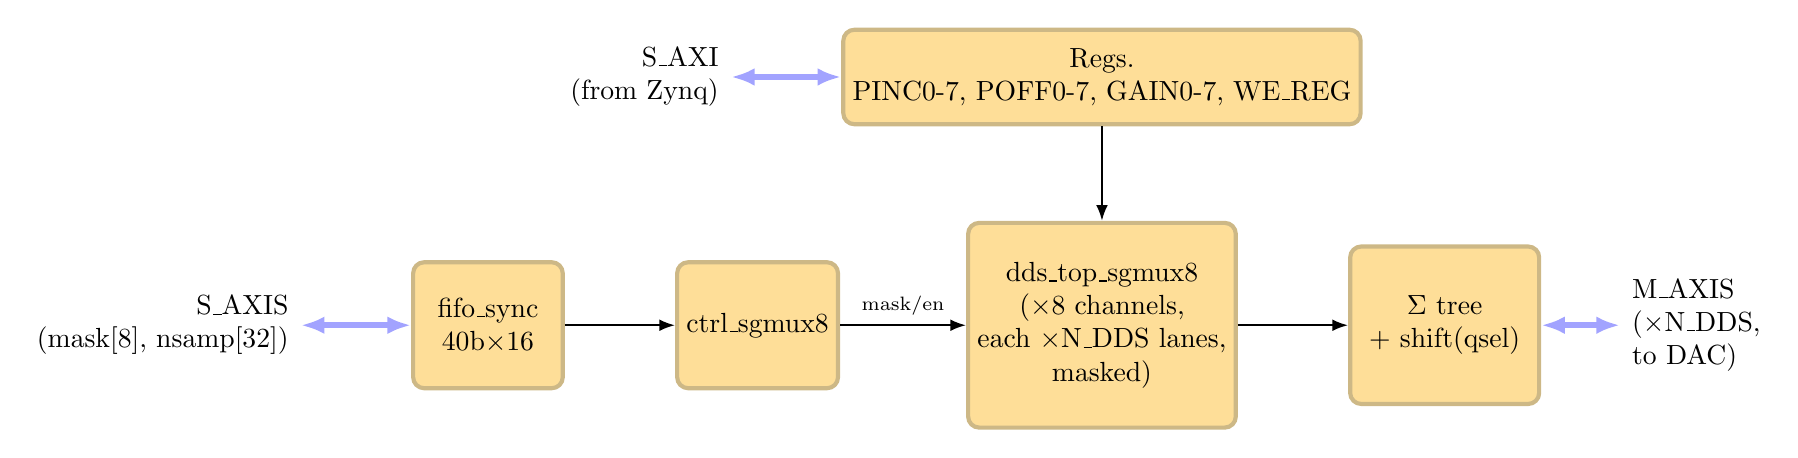
\begin{tikzpicture}
[box/.style={align=center, draw,rounded corners,minimum width=1.9cm,minimum height=1.2cm,draw={rgb,255:red,205; green,184; blue,134},fill={rgb,255:red,254; green,222; blue,152},line width=1.5pt},
arrow/.style={line width=2.2pt,draw={rgb,255:red,162; green,163; blue,255},{Latex[length=3mm]}-{Latex[length=3mm]}},
single arrow/.style={line width=0.8pt,-{Latex[length=2mm]}},
node distance=0.4cm]

% Fifo.
\node[box,minimum height=1.6cm] (fifo) {fifo\_sync\\40b$\times$16};

% Control.
\node[box,right=1.4cm of fifo,minimum height=1.6cm] (ctrl) {ctrl\_sgmux8};

% DDS array (8 masked channels).
\node[box,right=1.6cm of ctrl,minimum height=2.6cm,minimum width=3.2cm] (dds) {dds\_top\_sgmux8\\ ($\times$8 channels,\\ each $\times$N\_DDS lanes,\\ masked)};

% Adder tree + quantization.
\node[box,right=1.4cm of dds,minimum height=2cm,minimum width=2.4cm] (sum) {$\Sigma$ tree\\ + shift(qsel)};

% Regs.
\coordinate (temp) at ($(dds.north)+(0,1.2)$);
\node[box,anchor=south,minimum width=5cm] (regs) at (temp) {Regs.\\PINC0-7, POFF0-7, GAIN0-7, WE\_REG};

% s_axis: waveform descriptor.
\draw[arrow] ($(fifo.west)+(-1.4,0)$) coordinate (s axis in) node[anchor=east,align=right] {S\_AXIS\\(mask[8], nsamp[32])} -- (fifo.west);

% s_axi (registers), from Zynq.
\draw[arrow] ($(regs.west)+(-1.4,0)$) coordinate (temp) node[anchor=east,align=right] {S\_AXI\\(from Zynq)} -- (regs.west);

% fifo -> ctrl.
\draw[single arrow] (fifo.east) -- (ctrl.west);

% ctrl -> dds (mask/en).
\draw[single arrow] (ctrl.east) -- (dds.west) node[pos=0.5,above,font=\scriptsize] {mask/en};

% Regs -> dds (PINC/POFF/GAIN).
\draw[single arrow] (regs.south) -- (regs.south |- dds.north);

% dds -> sum.
\draw[single arrow] (dds.east) -- (sum.west);

% m_axis.
\draw[arrow] (sum.east) -- ++(1,0) node[anchor=west,align=left] {M\_AXIS\\($\times$N\_DDS,\\ to DAC)};

\end{tikzpicture}

\end{document}
